\documentclass[border=5pt]{standalone}
\usepackage{tikz}
\usetikzlibrary{calc}
\begin{document}
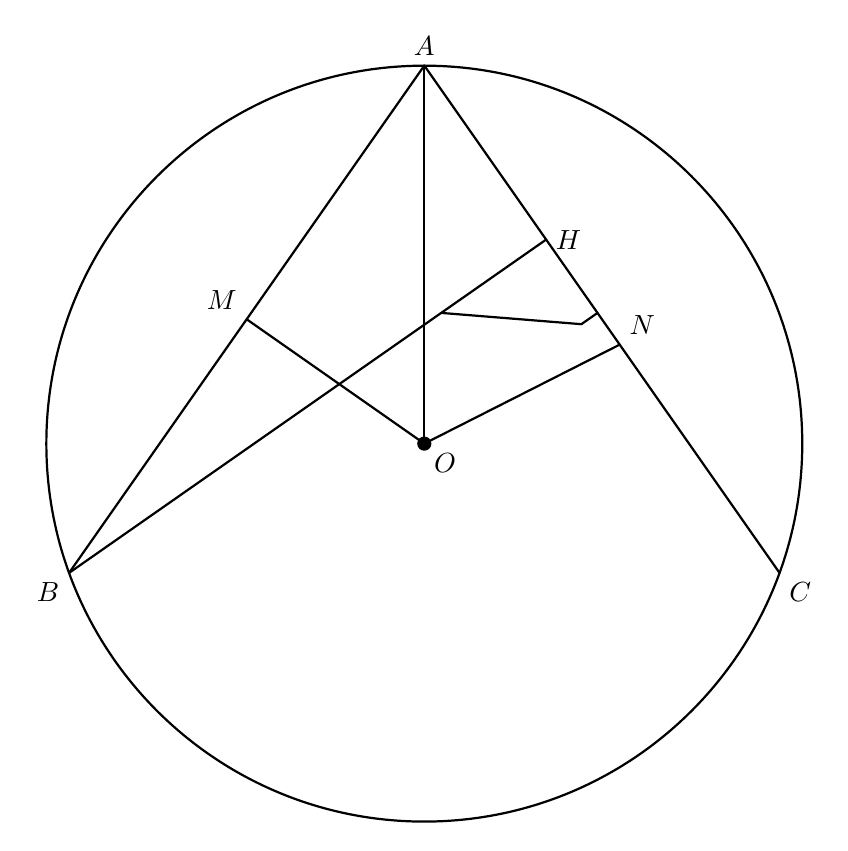
\begin{tikzpicture}[scale=1.6,line cap=round,line join=round]
  % Circle and center
  \coordinate (O) at (0,0);
  \draw[thick] (O) circle (3);
  \fill (O) circle (1.6pt);

  % Points on circle
  \coordinate (A) at (90:3);
  \coordinate (B) at (200:3);
  \coordinate (C) at (340:3);

  % Foot of perpendicular from B to AC
  \coordinate (H) at ($(A)!0.343!(C)$);

  % Midpoints
  \coordinate (M) at ($(A)!0.5!(B)$);
  \coordinate (N) at ($(A)!0.55!(C)$);

  % Triangle and segments
  \draw[thick] (B) -- (A) -- (C);
  \draw[thick] (A) -- (O);
  \draw[thick] (O) -- (M);
  \draw[thick] (O) -- (N);
  \draw[thick] (B) -- (H);

  % Right angle mark at H
  \begin{scope}
    \coordinate (u1) at ($(H)!0.22!(C)$);
    \coordinate (u2) at ($(H)!0.22!(B)$);
    \draw[thick] ($(H)!0.22!(C)$) -- ($($(H)!0.22!(C)$)!0.22!90:(H)$) -- ($(H)!0.22!(B)$);
  \end{scope}

  % Labels
  \node[above] at (A) {$A$};
  \node[below left] at (B) {$B$};
  \node[below right] at (C) {$C$};
  \node[below right] at (O) {$O$};
  \node[above left] at (M) {$M$};
  \node[above right] at (N) {$N$};
  \node[right] at (H) {$H$};
\end{tikzpicture}
\end{document}
